%**************************************************
% Einführung in die Empirische Wirtschafftsforschung Formelsammlung
% First version by Paul Gruenenwald
%**************************************************


% Use extarticle for the smaller font size:

\documentclass[a3paper, 8pt]{extarticle}

% Multi-column layout
\usepackage{multicol}

\usepackage{pgfplots}
\usepgfplotslibrary{fillbetween}

% Manually set page margins
\usepackage[margin=0.5cm, bmargin=0.8cm, landscape]{geometry}

\usepackage{multirow}
\usepackage{titlesec}
\usepackage[parfill]{parskip}
\usepackage{enumitem}
\usepackage[document]{ragged2e}
\usepackage[nodisplayskipstretch]{setspace}
\setstretch{1}
\setlist{leftmargin = 4mm, nosep}
% or \setlist{noitemsep} to leave space around whole list
%create new list type
\newlist{mylist}{enumerate}{4}

\titleformat{\section}
[block]
{\RaggedRight \fontsize{12}{12}\sc}
{\thesection}
{5pt}
{}
[\vspace{0.5pt}\hrule\vspace{1pt}]

\titleformat{\subsection}
[block]
{\RaggedRight \fontsize{10}{10}\sc}
{\thesubsection}
{4pt}
{}
[\vspace{0.5pt}\hrule \vspace{1pt}]


\titleformat{\subsubsection}
[block]
{\RaggedRight \fontsize{10}{10}}
{\thesubsubsection}
{4pt}
{}
[\hrule \vspace{4pt}]
%Defining a Definition for proofs and stuff

\titleformat{\paragraph}
[runin]
{\RaggedRight \bf}
{}
{}
{}
[]

\titlespacing{\paragraph}{}{3pt}{5pt}

\titlespacing{\subsubsection}{0pt}{8pt}{0pt}

\usepackage{amsmath}

\usepackage{amsthm}
\newtheorem{theorem}{Theorem}
\newtheorem{corollary}{Corollary}[theorem]
\newtheorem{lemma}[theorem]{Lemma}

\newtheorem*{definition}{Definition}

\newtheorem*{remark}{Remark}


\usepackage{mathtools}
\usepackage{amssymb}
\usepackage{graphicx}
\usepackage[english]{babel}
\usepackage{blindtext}

\usepackage{graphicx}
\graphicspath{ {./graphics/} }

\begin{document}
\setlength{\abovedisplayskip}{6pt}
\setlength{\belowdisplayskip}{6pt}
\setlength{\abovedisplayshortskip}{5pt}
\setlength{\belowdisplayshortskip}{5pt}


\RaggedRight


\begin{multicols*}{5}

\subsubsection{Kennzahlen}
\paragraph{Erwartungswert}
    $E(x)=\Sigma_i x_i p_i$

\paragraph{Zufallsvariable}
 
\paragraph{Standardfehler} $SF$ The standard error of the model, denoted by s, is our estimate of the standard deviation of the noise in Y. Zwischen verschiedenen Stichproben. Wie stark die Mittelwert dieser Stichproben voneinander abweichen.

    
\paragraph{Standardabweichung} $s= \sqrt{\frac{1}{n-1}\Sigma_{i=1}^n (x_i - \bar{x})^2}$\\ Innerhalb einer Stichprobe wie sehr konkrete Werte vom Mittelwert dieser Stichprobe abweichen.
Das Symbol der Standardabweichung für eine Zufallsvariable wird mit „$\sigma$“ angegeben, das für eine Stichprobe mit „s“.
 

\paragraph{Varianz}
Grundgesamtheit $s^2 = \frac{1}{n}\Sigma_{i=1}^n (x_i - \bar{x})^2$\\
Stichprobe $s^2 = \frac{1}{n-1}\Sigma_{i=1}^n (x_i - \bar{x})^2$

\paragraph{Freiheitsgrade} $N-\#$ Variablen ($X$ \& $Y$ sind Variablen)

\paragraph{Parameter} Koeffizienten, die verschieden Werte annehmen können.

\texttt{9.1093822e-9} $= 9.1093822\cdot 10^{-9}$


\paragraph{Konsistenz} für einen zu schätzenden Parameter der Grundgesamtheit, wenn die Folge von Schätzfunktionen mit steigendem Stichprobenumfang n gegen den Parameter stochastisch konvergiert (schwache Konsistenz), d.h., dass die Wahrscheinlichkeit, dass sich der Parameter und der Schätzwert um mehr als eine beliebig kleine positive Größe unterscheiden, mit wachsendem Stichprobenumfang gegen 0 geht (s. Gesetze der großen Zahlen).

\paragraph{Querschnittsdaten} sind das Ergebnis von Datenerhebungen, die nur zu einem Zeitpunkt an einer statischen Einheit durchgeführt werden.

In R $t_0-wert=\frac{b_0}{SF(b_0)}$ und $t_1-Wert=\frac{b_1}{SF(b_1)}$ Entspricht einfach dem z-wert nur dass dieser auch für kleinere Stichproben gilt.
\subsubsection{Bedingte Wahrscheinlichkeit}
$P(A|B)=\frac{P(A\cap B)}{P(B)}=\frac{P(A, B)}{P(B)}$


\paragraph{Konfidenzniveaus}

\begin{center}
\begin{tabular}{ c | c | c | c}
 Kon. Niv. $1-\alpha$ & 90\% & 95\% & 99\% \\ \hline 
 Konstante $Z_{1-a/2}$ & 1.645 & 1.960 & 2.576
\end{tabular}
\end{center}

\subsubsection{Fehlertypen}
\pgfmathdeclarefunction{gauss}{3}{%
  \pgfmathparse{1/(#3*sqrt(2*pi))*exp(-((#1-#2)^2)/(2*#3^2))}%
}
\begin{center}
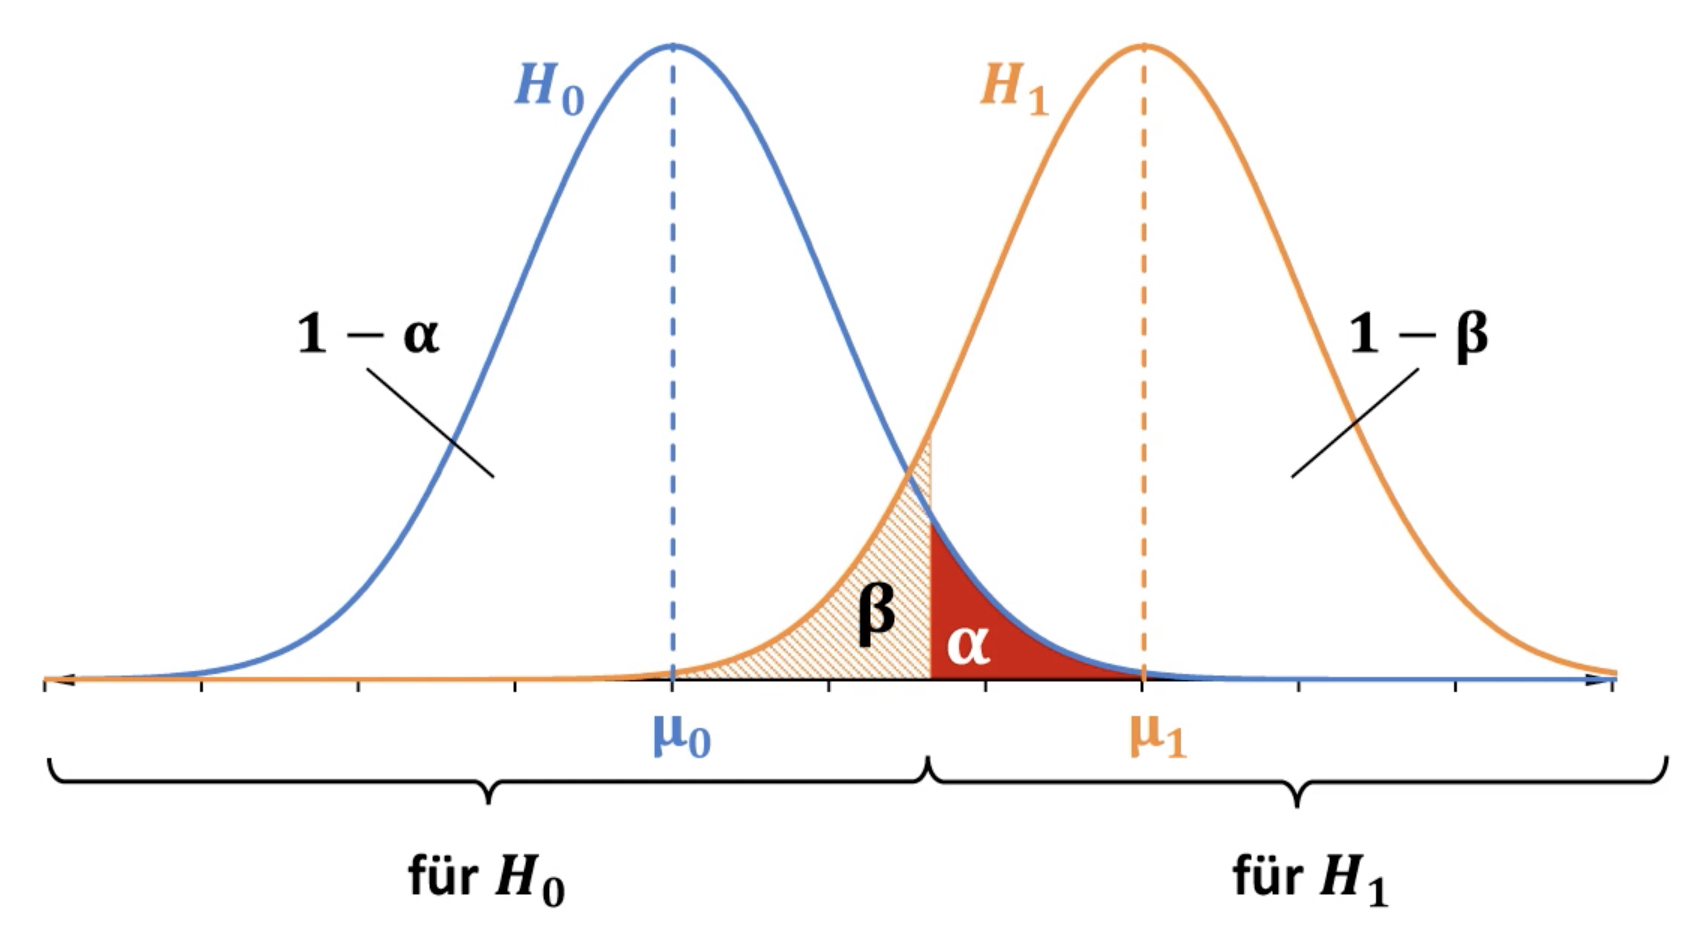
\includegraphics[width=0.8\columnwidth]{Untitled 2.jpg}
\end{center}

    
\begin{center}
\begin{tabular}{ c | c | c }
 $H_0$ & $H_0$ richtig & $H_0$ falsch\\ \hline 
 verwerfen & Typ I / $\alpha$-Fehler & richtig \\
 n. verwerf. & richtig & Typ II/ $\beta$-Fehler
\end{tabular}
\end{center}

\section{ Multivariate Statistik}
\paragraph{} Im Gegensatz zur univariaten Statistik, welche eine einzige Variable untersucht, werden in der  \textbf{multivariaten Statistik} mehrere (Zufalls-) Variablen gleichzeitig untersucht.
\paragraph{} Die \textbf{multivariate Verteilung} eines $d$-dimensionalen Zufallsvektors $X=(X_1,...,X_d)^T$, dessen Elemente alle Zufallsvariablen sind, ordnet jeder Teilmenge $A \subseteq R^d$ die Wahrscheinlichkeit zu, dass $X$ in Wert aus $A$ annimmt.\\

   
Eine multivariate Verteilung ist eine Verteilung von mehreren Zufallsvariablen. Sie ist das höherdimensionale Pendant zu einer univariaten Verteilungsfunktion.

\subsection{Gemeinsame Verteilungen}

\begin{center}
    \begin{tabular}{c|c|c|c}
         & Tot & Überlebt &   \\\hline 
        Mann & 0.64 & 0.16 & 0.8\\ \hline 
        Frau & 0.08 & 0.12 & 0.2 \\ \hline 
        & 0.72 & 0.28 & 1
    \end{tabular}
\end{center}
    

    \subsubsection{Gemeinsame W'keitsfunktion}{} Die gemeinsame Verteilung von zwei \textit{diskreten} Zufallsvariablen  $p(x,y)$ beschrieben:
    $P(X=x, Y=y) = p(x,y)$ \\
    \text{subject to:} $0 \leq p(x,y) \leq 1$ \\
    $\Sigma_x \Sigma_y \; p(x,y) = 1$
    
 
    \subsubsection{Gemeinsam Dichtefunktion} Die gemeinsame Verteilung von zwei \textit{stetigen} Zufallsvariablen $p(x,y)$ beschrieben:
    \begin{align*}
        P(a \leq X \leq b, c \leq Y \leq d) &= \int_a^b \int_c^d f(x,y)\; dy \; dx \\
        s.t. \:\:\: f(x,y) &\geq 0 \\
        \int_x \int_y f(x,y) \; dy \; dx &= 1
    \end{align*}
    
\paragraph{Bivariate Normalverteilung}
    Normalverteilungen können addiert werden.
    
\paragraph{Dachverteilung}
\begin{align*}
f(x,y)=
\begin{cases}
x+y & \text{für} \;0 \leq x\leq 1, 0 \leq y\leq 1\\
0 & \text{sonst}
\end{cases}
\end{align*}
    
\subsection{Randverteilungen} 
auch Marginalverteilung beschreibt die Verteilung einer Teilgruppe von Zufallsvariable einer Multivariaten Verteilung ohne Berücksichtigung der anderen Zufallsvariablen.
\begin{enumerate}
    \item[] \textit{Diskret} $P(X=x)=\Sigma_y p(x,y)$
    \item[] \textit{Stetige} $f(x) = \int_y f(x,y)\;dy$
\end{enumerate}

\subsection{Unabhängigkeit} 
Zwei Zufallsvariablen heissen unabhängig, wenn die Verteilung der einen Zufallsvariable nicht durch die andere Zufallsvariable beeinflusst werden.\\
Die Unabhängigkeit von Zufallsvariablen kann bei gegebenen Verteilungen mithilfe der Multiplikationsregel oder bei Datensätzen mithilfe eines Chi-Quadrat-Tests überprüft werden.

\paragraph{Multiplikationsregel}
 $$\textit{Diskret }p(x,y)=p(x)\;p(y)$
 $$\textit{Stetig }f(x,y)=f(x)\;f(y)$$

\subsubsection{Chi-Quadrat-Test}
Ist ein Unabhängigkeitstest ist eine Art des Hypothesentests, der für zwei diskrete Zufallsvariablen angewendet wird, um deren Unabhängigkeit zu überprüfen.
\vspace{2pt}
\begin{enumerate}
    \item Überprüfen Sie, dass $N \geq 50$ und legen Sie das Signifikanzniveau fest.
    \item Bestimmen Sie die erwarteten Häufigkeiten $(H_{jk})$ unter Unabhängigkeitsannahme: \\$H_{jk}=P(X=j)\times(Y=Kk)\times N$
    \item Berechnen Sie den Chi-Quadrat Wert mithilfe der tatsächlichen Häufigkeiten: \\
    $x^2=\Sigma_{j=1}^J \Sigma_{k=1}^K \frac{(h_{jk}-H_{jk})^2}{H_{jk}}$
    \item Berechnen Sie den Freiheitsgrad Ihrer Tabelle: \\
    $df =$ (Anzahl Zeilen - 1) × (Anzahl Spalten - 1)
    \item Vergleichen Sie Ihren Chi-Quadrat Wert mit dem kritischen Wert aus der Chi-Quadrat Tabelle
\end{enumerate}

%\paragraph{Kontingenztabelle}




\subsection{Bedingte Verteilung}
beschreibt die Verteilung einer Zufallsvariable mit der Voraussetzung, dass eine andere Zufallsvariable einen bestimmten Wert annimmt.
\vspace{3pt}
\begin{enumerate}
    \item[] \textit{Diskrete Zuffallsvariablen:} $p(x|y)=\frac{p(x,y)}{p(y)}$
    \item[] \textit{Stetige Zuffallsvariablen:} $f(x|y)=\frac{f(x,y)}{f(y)}$
\end{enumerate}


\subsubsection{Bedingte Verteilung: Unabhängigkeit}Bei zwei unabhängigen ZVn ist die jeweilige bedingte Verteilung gleich der jeweiligen Randverteilung:    \vspace{3pt}\\
    $$f(x|y)=\frac{f(x,y)}{f(y)}=\frac{f(x)f(y)}{f(y)}=f(x)$$
    
\subsection{Bedingter Erwartungswert}
$E(Y|x)$ ist der Erwartungswert einer bedingten Verteilung: \begin{align*}
   \textit{Stetig: } & E(Y|X=x)=\int y\;f(y|x)\;dy\\
\textit{Diskret: } & E(Y|X=x)=\Sigma_y \ y \cdot \frac{P(Y=y, X=x)}{P(X=x)}
\end{align*}

$E(X|Y)=\Sigma^n_{i=0} E(X|Y=y_i)\cdot P(Y=y_i) \cdot E(X)$


\subsubsection{Bedingter Erwartungswert: Unabhängigkeit} Bei Unabhängigkeit zweier ZV entspricht der bedingte Erwartungswert dem unbedingten Erwartungswert.
$$\text{Unabhängigkeit }\implies E(Y|x) = E(Y)$$
$$ \text{Aber }E(Y|x) = E(Y) \nRightarrow \text{Unabhängigkeit}$$

\subsection{Kovarianz und Korrelation}

 \paragraph{Varianz (Univariat)} $ \sigma^2 = E(X^2) - [E(x)]^2$


\paragraph{Kovarianz} beschreibt den linearen Zusammenhang zweier Zufallsvariablen. Der Wertebereich der Kovarianz erstreckt sich von minus unendlich bis plus unendlich.
\vspace{-3pt}
\begin{align*}
    Cov(X,Y) &= E[(X-(X))\;(Y-E(Y))]\\
    &= E[(X-E(X))\;Y]-E(X-E(X))\;E(Y)\\
    &= E(XY)-E(X)\;E(Y)
\end{align*}
Wenn die W’keit im Nordostquadranten oder im Südwestquadranten zu liegen höher ist, als die der anderen Bereiche, dann ist die Kovarianz positiv. Zudem werden Punkte weit
weg vom Schwerpunkt $(E(X), E(Y))$ stärker gewichtet.

Kovarianz zwischen zwei variablen, für den Fall von Stichproben wird geschrieben als $s_{x,y}$ oder $s_{y,x}$ ist definiert als \[s_{x,y}=\frac{\Sigma_{i=1}^N(X_i-\bar{X})(Y_i-\bar{Y})}{N-1}\]
\paragraph{Eigenschaften Kovarianz}
\begin{enumerate}
    \item Symmetrie: $$Cov(X, Y) = Cov(Y, X)$$
    \item Varianz = Kovarianz einer Variable mit sich selbst: $$Cov(X, X) = \sigma^2$$
    \item Wenn Erwartungswert von $X$ oder $Y = 0$, dann gilt: $$Cov(X, Y) = E(XY)$$
    \item Distributivgesetz: $$Cov(X + Y, Z) = Cov(X, Z) + Cov(Y, Z)$$
 $$Cov(a+bX,c+dY)=b\,d\;Cov(X,Y)$$
\end{enumerate}
 \vspace{5pt}

\paragraph{Unabhängigkeit} Wenn zwei ZV unabhängig sind ist die Kovarianz = 0. Die Umkehrung gilt jedoch \textbf{nicht}!

\paragraph{Problem} Die Kovarianz ist eine nicht-standardisierte Kennzahl. Dies impliziert, dass verschiedene Kovarianzen nicht miteinander verglichen werden können. Lösung: Korrelation = standardisierte Kovarianz

\paragraph{Korrelation} Ist die standardisierte Kovarianz. Ihr Wertebereich liegt zwischen -1 und +1.

$Corr(X,Y)=\frac{Cov(X,Y)}{\sigma_x \sigma_y}$
\begin{enumerate}
    \item[] $(\rho =1)$: Perfekt positive Korrelation
    \item[] $(0<\rho <1)$: Positive Korrelation
    \item[] $(1- < \rho < 0)$: Negative Korrelation
    \item[] $(\rho =-1)$: Perfekt negative Korrelation
\end{enumerate}
\vspace{3pt}
$Corr(X,Y)=\rho_{XY} = Cov [(\frac{X-E(X)}{\rho_X)},\frac{Y-E(Y)}{\rho_Y})]=\frac{Cov(X,Y)}{\rho_x \rho_Y}$

standardabweichung!

\paragraph{Stichprobenkovarianz}
$$\widehat{Cov}(X,Y) = s_{xy} = \frac{1}{N-p-1} \Sigma_{i=1}^N (x_1- \bar{x})(y_i - \bar{y})$$
$p:$ Anzahl der Regressoren. 
\paragraph{Populationskovarianz}
$$\widehat{Cov}(X,Y) = s_{xy} = \frac{1}{N-p} \Sigma_{i=1}^N (x_1- \bar{x})(y_i - \bar{y})$$

\paragraph{Stichproben Korrelation}
$$r_{xy}=\frac{\widehat{Cov}(X,Y)}{s_x s_y}=\frac{s_{xy}}{s_x s_y}$$\\
$s_x$ ist die Stichproben(standard)abweichung von $X$ und $s_y$ die von $Y$



\section{Statistische Modelle für Y}
\paragraph{Inputs $X$} bezeichnet die Menge der Variable, welche die Ausprägung des Outputs $Y$ beeinflussen. $X$ hat verschiedene Bezeichnungen: \textit{Prediktoren, Ausgangsvariablen, unabhängige Variablen, erklärende Variablen, Regressoren, Features.}

\paragraph{Outputs $Y$} bezeichnet diejenige Variable, welche durch $X$ beeinflusst wird. Bezeichnungen für $Y$ sind zB.: \textit{Zielvariable, Zielgrösse, abhängige Variable}

\subsubsection{$Y$ als Funktion von $X$}
$Y=f(X) + \epsilon$\\
$\epsilon$ = Unreduzierbarer Fehler\\

Wir können immer schreiben:\\
$Y=\beta_0+\beta_1X+f(X)-\beta_0-\beta_1X+\epsilon$ \\bzw. $Y=\beta_0+\beta_1X+u$\\
$u$: Gesamtfehler (Approximationsfehler + $\epsilon$)\\
Approximationsfehler: $f(X)-\beta_0-\beta_1X$

%\subsection{Die Funktion $f(X)$}

\subsection{Inferenz}
Das Ziel der \textbf{statistischen Inferenz} ist Aussagen über die Beziehung von $Y$ und $X$ in einer Population mithilfe der Stichprobe zu tätigen. Dabei wird die geschätzte Funktion $f(X)$ interpretiert.

\paragraph{Inferenzfragen} Die statistische Inferenz erlaubt es, mittels einer Stichprobe Aussagen bzw. Schlussfolgerungen über die Population zu tätigen.

\subsection{Prognose}
Mit einer \textbf{Prognose} wird in der Statistik versucht, anhand von historischen Daten, Aussagen über zukünftige Ereignisse zu treffen.

\paragraph{Prognosefehler} $Y - \hat{Y}$ beschreibt die Differenz zwischen dem tatsächlichen unde dem erwarteten Wert eines Ereignisses.
$$Y - \hat{Y} = f(X)- \hat{f}(X) + \epsilon$$
\begin{itemize}
    \item Reduzierbarer Fehler $f(X)-\hat{f}(X)$
    \item Unreduzierbarer Fehler $\epsilon$
\end{itemize}
   
\paragraph{Mittlerer quadratischer Progonosefehler} oder \textit{Mean squared error} (MSE). Ist der Mittelwert aller quadrierten Distanzen zsichen der Schätzfunktion $\hat{f}(X)$ und den Tatsächlichen Werten. Es wird unterschieden zwischen Training-MSE und Test-MSE. Da Prognosefehler positiv oder negativ sein können werden diese vergleichbar gemacht.

\[MSE=\frac{1}{N}\Sigma_{i=1}^N(y_i-\hat{y}_1)^2\]
\begin{align*}
    E(Y-\hat{Y})^2 =& E[f(x)+\epsilon-\hat{f}(X)]^2\\
=& E[f(x)-\hat{f}(X)]^2 + Var(\epsilon)
\end{align*}

\paragraph{Herkunft des unreduzierbaren Fehlers $\epsilon$}\begin{itemize}
    \item unberücksichtigte Inputvariablen
    \item unberücksichtigte, zufällige Variation in der Funktion $f$
\end{itemize}



\subsection{Ansätze zur Schätzung von $f(X)$}

\subsubsection{Parametrische Modelle}
Bei einem parametrischen Modell sind alle Informationen in den Parametern enthalten. Dazu wird eine spezielle Funktion angenommen (oft: linear):
\[f(X)=\beta_0+\beta_1X\]
Zu bestimmende Parameter:
\begin{enumerate}
    \item[] $\beta_0$: Achsenabschnitt (Intercept)
    \item[] $\beta_1$: Steigung (Slope)
\end{enumerate}

\subsubsection{Nicht-parametrische Modelle}Ein nicht-parametrisches Modell ist ein parameterfreies statistisches Modell, bei dem keine Voraussetzungen bezüglich der Struktur bestehen und diese erst aus den Daten bestimmt wird. Nicht-parametrische Modelle sind viel flexibler.

\paragraph{KNN ($K$-Nearest Neighbors)}
Für jeden Punkt $x_0$ finden wir die $K\:x_i$-Werte die $x_0$ am nächsten liegen. Die Menge dieser $x$-Werte nennen wir $N_0$. Der Schätzer für $f(x_0)$ ist der Durchschnitt aller $y_i$ Werte für $x_i \in N_0$

\subsubsection{Semiparametrische Modelle}
Semiparametrische Modelle haben sowohl parametrische als auch nicht-parametrische Komponenten. Sie sind meist flexibler als parametrische Modelle und gleichzeitig simpler als nicht-parametrische Modelle.Beispiel, Polynom höherer Ordnung:
\[f(X)=\beta_0+\beta_1X+\beta_2X^2+ \dots \beta_nX^n\]

\subsection{Güte der Anpassung} zeigt, wie gut ein Modell die Beobachtungen erklären kann. Sie wird allgemein mit dem Mean-Squared Error zwischen Beobachtung von $Y$ und Prognosewert $\hat{Y}$ gemessen.

\paragraph{Training-Daten} beschreibt die Daten, welche bereits im Datensatz enthalten sind und mit denen ein Modell "trainiert" wird.

\paragraph{Test-Daten} beschreibt die Daten, welche in neuen Beobachtungen enthalten sind und mit denen ein Modell "getestet" wird.

\subsubsection{Training-MSE}
misst den Fehler für die (beobachteten) Training- Daten. Er ist ein Mass für den "in-sample" (="training data") Fit.
\[MSE_{\text{training}} = \frac{1}{N}\Sigma_{i=1}^N (y_i-\hat{f}(x_i))^2\]

\begin{enumerate}
    \item[]$y_i$: tatsächlicher Wert (Training-Daten)
    \item[]$f(\hat{x}_i)$: geschätzter Prognosewert
    \item[]$N$: Anzahl Beobachtungen, die zur Scätzung von $\hat{f}$ verwendet wurden.
\end{enumerate}

\subsubsection{Test-MSE}
misst den Fehler auf den (neuen, zukünftigen) Test-Daten. Der Test-MSE ist ein Mass für den "out-of-sample" (="test data") Fit.
\[MSE_{\text{test}} = \frac{1}{\Tilde{N}}\Sigma_{j=1}^{\Tilde{N}} (y_j-\hat{f}(x_j))^2\]

\begin{enumerate}
    \item[]$y_j$: tatsächlicher zukünftiger Wert (Test-Daten)
    \item[]$\hat{f}(x_j)$: aufgrund d. Training-Daten geschätzter Wert
    \item[]$\Tilde{N}$: alle neuen Beobachtungen, mit denen die Schätzung $\hat{f}$ getestet wird
\end{enumerate}
\subsubsection{Overfitting}
Beim Overfitting hat ein komplexes Model einen niedrigeren Training-MSE, jedoch einen höheren Test-MSE.
 

\section{Lineare Einfachregression} 
\subsection{Das lineare Regressionsmodell}
Schätzt eine lineare Beziehung zwischen Prediktor(en) und Output.
\[Y=\beta_0+\beta_1X+\epsilon\]

\begin{enumerate}
    \item[] $\beta_0, \beta_1$: Parameter / Regressionskoeffizienten
    \item[] $\beta_0$: Achsenabschnitt (Intercept)
    \item[] $\beta_1$: Steigung (Slope)
    \item[] $\epsilon$: (stochastischer) Fehler
    \item[] $X$: Input
    \item[] $Y$: Output
\end{enumerate}

\subsubsection{Fehlerannahmen}

\paragraph{Annahme Erwartungswert:}\begin{itemize}
    \item Wenn $X$ nicht zufällig: $E(\epsilon) = 0$
    \item Wenn $X$ zufällig: $E(\epsilon | X)=0$
\end{itemize}

\paragraph{(Fehlervarianz)} Evtl. nut bedingt gültig $Var(\epsilon)=\sigma^2$ ist ein Mass dafür, wie weit die Y-Werte im Durchschnitt von der Regressionslinie entfern sind: Wir nehmen an, dass sie konstant ist.

\paragraph{Korrelation der Fehler} Die Fehlerterme sind unkorreliert: $Cor(\epsilon_i,\epsilon_j)=0, \: i\neq j$

\subsection{Geschätztes Modell}
Die wahren Werte für $\beta_0$ und $\beta_1$ sind unbekannt. Das \textbf{geschätzte Modell} versucht, diese Parameter möglichst akkurat zu schätzen.
\[\hat{Y}=b_0+b_1X\]
\begin{enumerate}
    \item[] $\hat{Y}$: geschätzter Regressionswert / Prognosewert
    \item[] $b_0, b_1$: geschätzte Parameter Schätzer (werden auch als $\hat{\beta}_0, \hat{\beta}_1$ notiert)
\end{enumerate}

\subsubsection{Residuum}
Das Residuum am Punkt $x_i$ für das geschätzte Modell ist die Differenz zwischen tatsächlichem und dem gemäß Modell zu erwartenden Werts:
\begin{align*}
    e_i &=y_i - \hat{y}(x_i)\\
    &= y_i-b_0-b_1x_i
\end{align*}

\subsubsection{Kleinste-Quadrate Methode}
Ist ein Verfahren zur Ermittlung des geschätzten Models, das die Werte bestmöglich fittet. Bei der KQ Methode minimieren wir den MSE bzw. gleichbedeutend, die Summe der quadrierten Residuen.

\paragraph{Herleitung}
\begin{enumerate}
    \item Minimierungsproblem aufstellen:\\ $\underset{b_0,b_1}{\text{min}}\frac{1}{N}\Sigma_{i=1}^N(y_i-\hat{y}_i)^2 $
    \item Konstante $1/N$ kürzen und das Minimierungsproblem umformen: $\text{min}\Sigma_{i=1}^N(y_i-b_0-b_1x_i)^2$
    \item Bedingungen erster Ordnung aufstellen:\\
    $\frac{\delta SQR}{\delta b_0}=-2 \Sigma_{i=1}    ^N(y_i-b_0-b_1x_i)=0$\\
    $\frac{\delta SQR}{\delta b_1}=-2 \Sigma_{i=1}    ^N(y_i-b_0-b_1x_i)=0$
    \item Erste Gleichung nach $b_0$ auflösen: $b_0=\bar{y}-b_1\bar{x}$
    \item Einsetzen von $b_0$ in die zweite Gleichung
    \item Nach $b_1$ umformen
    \item ...
\end{enumerate}

\paragraph{SQR}Summe der quadrierten Residuen (RSS, residual sum of squares): $SQR=\Sigma_{i=1}^Ne_i^2 \: = \:\Sigma_{i=1}^N(y_i-\hat{y}_i)^2$

\subsubsection{KQ Methode Ergebnis}
\paragraph{Achsenabschnitt} $b_0 = \bar{y}-b_1\bar{x}$

\paragraph{Steigung}
$b_1 =\frac{\widehat{Cov}(Y,X)}{\widehat{Var}(X)}$

\paragraph{Unverzerrtheit} Damit die Schätzung $b_1$ des Steigungsparameters $\beta_1$ im linearen Modell $Y=\beta_0+\beta_1X+\epsilon\ $ unverzerrt ist (d.h: $$E(b_1)=\beta_1$$ muss gelten $E(\epsilon)=0$ 
%\subsubsection{Eigenschaften der Lösung}
%\subsubsection{Besonders einfache Einfachregression}

\subsection{Schätzvert. \& KI des KQ-Schätzers}
\subsubsection{Erwartungswert des KQ-Schätzers}
Die KQ Methode ergibt eine Schätzung für die wahre lineare Beziehung.
E$(b_0)= \beta_0$
E$(b_1) = \beta_1$

(Unverzerrtheit)

\subsubsection{Varianz des KQ-Schätzers} 

$$Var(b_0)=\sigma^2 \left( \frac{1}{N}+\frac{\Bar{x}}{\Sigma_{i=1}^N(x_i-\Bar{x})^2}\right)$$
$$Var(b_1)=\frac{\sigma^2}{\Sigma_{i=1}^N(x_i-\bar{x})^2}$$

\paragraph{Unverzerrter Schätzer für $\sigma^2$} Die Varianz von $\epsilon$ ist unbekannt, kann aber durch die Stichprobenvarianz der Residuen geschätzt werden:\\ $$\hat{\sigma}^2 \equiv s^2 = \frac{1}{N-1}\Sigma_{i=1}^N e_i^2 = \frac{SQR}{N-1}$$
Die Varianz des Fehlerterms bleibt unverändert in $N$. Unter der Annahme dass die Fehlerterme unkorreliert mit $X$ sind.
\subsubsection{Eigenschaften der Varianz der Schätzer}
\begin{itemize}
    \item Je mehr $x$ variiert, desto kleiner die Varianz von $b_1$
    \item Wenn $x_i$ konstant: $b_1$ lässt sixh nicht bestimmen
    \item Je grösser $N$, desto kleiner die Varianz von $b_1$
    \item Die Formeln der Varianz gelten nur, wenn: \begin{itemize}
        \item Die Fehler unabhänig sind
        \item die Fehler eine konstante Variianz haben
        \item Die Regressoren $X$ nicht-zufällig sind
    \end{itemize}
\end{itemize}

\subsubsection{Konfidenzintervall für $\beta$}
Für hinreichend grosse Stichproben (Regel $N-2>30$) gilt der Zentrale Grenzwertsatz: $$b \thickapprox Normal(\beta_1, \frac{\sigma^2}{\Sigma_{i=1}^N(x_i-\bar{x}^2})$$
$$SF(b_1)=\sqrt{\frac{\hat{\sigma}^2}{\Sigma_{i=1}^N(x_i-\bar{x})^2}}=\sqrt{\frac{SQR/(N-2)}{\Sigma_{i=1}^N(x_i-\bar{x})^2}}$$
Der Konfidenzintervall für $\beta_1$ wird zur Beurteilung der Schätzgenauigkeit der Parameter verwendet. E gibt die Konfidenz an, dass das wahre $\beta_1$ in einem bestimmten Intervall liegt. Hierbei handelt es sich um eine Intervallschätzung. Das 95\% KI für $$KI \ \beta_1: b_1 \pm 1.96 \times SF(b_1)$$
\subsection{Hypothesentest}
\begin{enumerate}
    \item In Abhängigkeit der relativen Kosten einer Fehlentscheidung $H_0$ und $H_1$ bestimmen
    \item Die maximal tolerierte Wahrscheinlichkeit für den Typ-I Fehler (Signifikanzniveau) festlegen, zB $\alpha = 0.05$ (Typ I Fehler: Obwohl $H_0$ zutrifft $H_0$ ablehnen)
    \item Prüfen: sind die Bedingunged für den ZGS erfüllt?
    \item Wert der Test-Statistik ($z$-Wert) bei Gültigkeit von $H_0$ berechnen
    \item $p$-Wert berechnen (Die W'keit unter $H_0$ den gegebenen $z-$Wert zu erhalten)
    \item $H_0$ auf dem $100 \times \alpha \%$ Signifikanzniveau (nicht) verwerfen
\end{enumerate}

\subsubsection{Hypothesentest für $\beta_1$}
Meistens wird geprüft, ob es eine Beziehung zwischen $X$ und $Y$ gibt. Die Hypothesen lauten dann: \begin{itemize}
    \item[$H_0$] Keine Beziehung zwischen $X$ und $Y$
    \item[$H_1$] Eine Beziehung zwischen $X$ und $Y$
    \item Zweiseitiger Test: $H_0: \beta_1 = 0$; $H_1: \beta_1 \neq 0$
    \item Teststatistik $z=\frac{b_1-\beta_{0,0}}{SF(b_1)}$
    \item p-Wert: $2P(Z > |z|)$ (wobei $Z=$ die standardnormalverteilte Zufallsvariable)
\end{itemize}
\subsection{Prognose $y_{neu}$}
Um $y_{neu}$ vorherzusagen, können wir eine Punktschätzung oder eine Intervallschätzung für den prognostizierten Wert machen

\subsubsection{Punktschätzung für $y_{neu}$} Wird mittel der geschätzten Regressionsgerade bestimmt: $\hat{y}_{neu}=b_0+b_1 x_{neu}$

\subsubsection{Intervallschätzung}
\paragraph{Intervallschätzung für $\mu_{neu}$} (Erwartungswert von $y_{neu}$): $\mu_{neu}=\beta_0+\beta_1 \: x_{neu}$ ergibt ein Konfidenzintervall, in dem der Erwartungswert von $y_{neu}$ ($\mu_{neu}$) mit einer bestimmten Konfidenz liegt.

\paragraph{Intervallschätzung für $y_{neu}$:} $$y_{neu} = \beta_0 + \beta_1 \: x_{neu} + \epsilon$$ ergibt ein Vorhersageintervall, in dem $y_{neu}$ mit einer bestimmten Konfidenz liegt.

\paragraph{Varianz der Prognose} 
Bei der Intervallschätzung wird die Unsicherheit der Schätzung durch den Standardfehler, bzw. durch die Varianz der Prognose quantifiziert. Die Varianz der Prognose wird als quadrierter SF der Prognose ausgedrückt:
$$\widehat{Var}(\hat{y}_{neu})= [SF(\hat{y}_{neu})]^2$$

\paragraph{Standardfehler der Prognose} $$SF(\hat{y}_{neu})=s\sqrt{\frac{1}{N}+\frac{(\bar{x}-x_{neu})^2}{\Sigma_{i=1}^N(x_i-\bar{x})^2}}$$ wobei $s$ das unbekannte $\sigma$ ersetzt. 

\paragraph{KI für $\mu_{neu}$:} 
$\hat{y}\pm z_{1-\frac{\alpha}{2}} \times SF(\hat{y}_{neu})$

\paragraph{Vorhersageintervall für $y_{neu}$}
gibt den Bereich an in dem \textit{einzelne Werte} mit vorgegebener Konfidenz liegen werden. Zusätzlich zu den Schätzfehlern bei $b_0$ und $b_1$ kommt noch die Variation von $\epsilon$ dazu.\\
Wir machein die einmalige Annahme: Die Fehler sind normalverteil.
$$\hat{y}_{neu} \pm z_{1-\frac{\alpha}{2}} \times s \sqrt{1+\frac{1}{N}+\frac{(\bar{x}-x_{neu})^2}{\Sigma_{i=1}^N(x_i-\bar{x})^2}}$$
Das Vorhersageintervall ist immer, und meist deutlich, grösser als das KI der Prognose.

\subsubsection{Extrapolation}
bezeichnet die Situation, in der eine Vorhersage für einen Wert $x_neu$ gemacht wird, der weit ausserhalb der $x$ Werte liegt, die zur Schätzung der Linie verwendet wurden. Solche Prognosen sind häufig sehr ungenau.
   
\subsection{Anpassungsgüte des linearen Modells}
zeigt, wie gut ein Modell die Beobachtungen erklären kann. Sie wird allgemein mit der Mittleren Quadratischen Abweichung \textbf{(Mean-Squared Error = MSE)} zwischen Beobachtung von $Y$ und Prognosewert $\hat{Y}$ gemessen. Wie wir sehen werden, kann sie aber auch mit anderen Kennzahlen gemessen werden.
\subsection{In-Sample}
\paragraph{SQR} Wenn die Summe der quadrierten Residuen Null ist, ist der Fit perfekt. Alle Datenpunkte liegen
auf einer Linie. $$SQR=\Sigma_{i=1}^N e^2_i=\Sigma_{i=1}^N (y_i-\tilde{f}(x_i))^2=\Sigma_{i=1}^N (y_i-\hat{y}_i)^2$$

\paragraph{Stichproben-MSE} $MSE=\frac{SQR}{N-2}=\hat{\sigma}^2$\\ Wobei $E(MSE)=\sigma^2$

\paragraph{RMSE} root-mean squared error (Standardfehler der Regression) gibt an, wie stark eine Prognose im Durchschnitt von den Daten abweicht:
$$RMSE=\sqrt{MSE}$$

\paragraph{$R^2$} Gibt an, wie viel der Variation von $Y$ durch die Variation von $X$ erklärt werden kann.
$$R^2=1-\frac{SQR}{TQS}=1-\frac{\Sigma_{i=1}^N e_i^2}{\Sigma_{i=1}^N(y_i-\bar{y})^2}$$

!!see above
%Totale Quadratsumme %$TQS=\Sigma_{i=1}^N(y_i-\bar{y})^2$ \\
$0 \leq R^2 \leq 1$
\subsection{Out-of-Sample (Prognosegüte)}
Es ist üblich die Daten in zwei Teile (2/3 Trainings-Daten und 1/3 Test-Daten) aufzuteilen.

\section{Mehrfachregression} 
\subsection{Lineare Mehfrachregression}
\subsubsection{Allgemeine Modell $REG_p$}
$Y=\beta_0+\beta_1X_1+\beta_2X_2+ \dots + \beta_pX_p+\epsilon$
\subsubsection{KQ Methode verallgemeinert}

Vorraussetzungen \begin{itemize}
    \item $p < N$
    \item $X_j$ und $X_k$ dürfen nicht in einem linearen Zusammenhang stehen
\end{itemize}

Implikation: Die Bedinungen 1. Ordnung für ein Minimum bedeuten: alle Prediktoren sind unkorreliert mit, bzw. orthogonal zu den Residuen.
\subsubsection{Ceteris paribus} Bedeutet "alles andere gleich"
$\Delta \hat{Y}=b_1\Delta X_1$ bzw. $$b_1=\frac{\Delta \hat{Y}}{\Delta X_1}$$ bei gegebenem $X_2, X_3, \dots , X_p$
Je nach Anwendung wird c.p. oft vorgezogen weil es der Idee eine \textit{kausalen Effektes} näher kommt.

\paragraph{Unerwünschter c.p.}


\subsubsection{SL: Multiple lineare Regression}

\subsection{Einfach- \& Mehrfachregression}
In diesem Teil werden die geschätzten Parameter der Einfachregression mit $g_0$ und $g_1$ bezeichnet:\\
\vspace{5pt}
$REG_1: Y=g_0+g_1X_1+u$\\
$REG_2: Y=b_0+b_1X_1+b_2X_2+e$

\subsubsection{Vergleich $REG_1$ \& $REG_2$}


Der KQ-Schätzer der Einfachregressions ($g_1$) kann durch die Schätzer der Zweifachregression ausgedrückt werden:
$$g_1=\frac{\widehat{Cov}(Y,X_1)}{\widehat{Var}(X_1)}=b_1+b_2 \cdot \frac{\widehat{Cov}(X_2,X_1)}{\widehat{Var}(X_1)}=b_1+b_2a_1$$
$a_1=\frac{\widehat{Cov}(X_1,X_2)}{\widehat{Var}(X_1)}$= Steigung der  "Hilfsregression" von $X_2$ auf $X_1$: $\hat{X}_2=a_0+a_1X_1$

%\paragraph{Herleitung} $\frac{\widehat{Cov}(Y,X_1)}{\widehat{Var}(X_1)}=b_1+b_2 \frac{\widehat{Cov}(X_1,X_2)}{\widehat{Var}(X_1)}$

\paragraph{Implikation} Im Allgemeinen gilt $g_1 \neq b_1$. Der geschätzte Effekt von $X_1$ auf $Y$ ist \textit{nicht} der gleiche in einer Einfachregression wie derjenige in einer (ceteris paribus) Mehrfachregression.

\paragraph{Ausnahme} $g_1=b_1$ wenn $\widehat{Cov}(X_2,X_1)=0$ bzw. $a_1=0$, also wenn $X_2$ und $X_1$ unkorreliert sin (oder wenn $b_2 = 0$)

\subsubsection{Regression \& Kausalität}
Eine Regression kann eine kausale Beziehung messen, muss es aber nicht! 

\paragraph{Was wir immer sagen können:}
$b_1$ gibt an, wie sich der Prognosewert $\hat{Y}$ ändert, wenn sich $X_1$ um eine Einheit erhöht und alle anderen $X$-Werte unverändert bleiben.

In der Realität gibt es viele Einflussfaktoren für eine Zielvariable $Y$.

\paragraph{Bedingungen für Kausalität}
\begin{itemize}
    \item $X$ ist vom Modellverständnis her eine mögliche Ursache von $Y$
    \item Alle Faktoren $X_2, \dots X_p$ die $Y$ ebenfalls kausal beeinflussen (und mit $X_1$ korrelieren), soweit beobachtbar, in die Mehrfachregression aufgenommen werden
    \item Alle unbeobachtbaren Faktoren, die unberücksichtigt bleiben, per Annahme nicht mit $X_1$ korrelieren
\end{itemize}

\paragraph{Unkorreliertheit sicherstellen} 
\begin{itemize}
    \item $X$ wird in einem Experiment randomisiert
    \item \textit{Kontrollvariablen-Methode:}Mehrfachregression durchführen, bei der möglichst alle weiteren potentiellen Einflussfaktoren aufgenommen werden und somit bei der Bestimmung von $b_1$ konstant gehalten werden. Die Annahme ist, dass der unbeobachtete Fehler $\epsilon$, der übrig bleibt, nachdem für $X_2, . . . , X_p$ kontrolliert wurde, nicht mehr mit $X_1$ korreliert.
\end{itemize}

Wenn die Annahme der Unkorreliertheit verletzt ist, dann gibt uns die Regression nicht den kausalen Effekt (“omitted variable bias”).

\paragraph{Scheinkorrelation} tritt auf, wenn zwei Variablen eine (hohe) Korrelation aufweisen und so ein statistisch existenter scheinbar kausaler Zusammenhang besteht, der jedoch nicht auf ein Ursache-Wirkungsprinzip zurückgeführt werden kann.

\paragraph{Selbstselektion}
beschreibt eine Form der willkürlichen Stichprobenziehung. Dabei entsteht eine Stichprobe, die einer vorhergehenden Selektion durch eine Person unterliegt, und so nicht mehr zufällig ist. Es handelt sich also um eine Wahlentscheidung, die von weiteren Umständen abhängt, die im Fehler εi enthalten sind.

\subsubsection{Residualvariation}
Die Residualvariation kann in der Regressionsanalyse dazu verwedet werden, die Koeffizienten einer Mehrfachregression durch wiederholte Anwendung von einer Einfachregression zu bestimmen, wobei der c.p. Effekt $b_1$ durch die c.p. Variation des Regressors $X_1$ geschätzt wird.

\paragraph{Beispiel} $REG_2: Y=b_0+b_1X_1+b_2X-2+e$
Für die Beziehung von $X_1$ und $X_2$ gibt es zwei Fälle:
\begin{enumerate}
    \item $X_1$ und $X_2$ sind unkorreliert: Dann gilt das Resultat der Äquivalenz ($g_1=b_1$)
    \item $X_1$ und $X_2$ korrelieren:\\ \textbf{Hilfsregression} Um die "Beziehung" zwischen $X_1$ und $X_2$ darstellen.
$\hat{X}_1=c_0+c_1X_2$
\\ \textbf{Interpretation} Wenn wir $Y$ auf $X_1-\hat{X}_1$ und $X_2$, statt auf $X_1$ und $X_2$ regressieren bekommen wir:\\ Der ceteris paribus Effekt $b_1$ wird durch ceteris paribus Variation des Regressors $X_1$ geschätzt. Dies ist Variation in $X_1$, die nicht mit $X_2$ korreliert also die Variation der Residuen der Hilfsregression
\end{itemize}

Der Mehrfachregressionskoeffizient $b_1$ kann ebenfalls mittels einer Einfachregression von $Y$ aud die Residuen $(X_1-\hat{X}_1)$  (statt auf $X_1 selber)$ bestimmt werden.

$X_1 - \hat{X}_1$ und $X_2$ sind per Konstruktion unkorreliert!

Modell\\
$REG_1: Y=g_0+g_1 X_1 + u$\\
$REG_2: Y=b_0+b_1 X_1 + b_2 X_2 + e$ \\
$REG_3: Y=b_0+b_1X_1+b_2X_2+b_3X_3+e$

$c$-Hilfsregression: $\hat{X}_1=c_0+c_1 X_2$\\
$a$-Hilfsreggression: $\hat{X}_2=a_0+a_1 X_1$
\renewcommand{\arraystretch}{1.3}

\begin{center}
    \begin{tabular}{l  l }
    $g_0$ & \texttt{lm(y $\sim$ x1)\$coefficients[1]} \\ \hline
    $g_1$ & \texttt{lm(y $\sim$ x1)\$coefficients[2]} \\ \hline
    $c_0$ & \texttt{lm(x1 $\sim$ x2)\$coefficients[1]} \\ \hline
    $c_1$ & \texttt{lm(x1 $\sim$ x2)\$coefficients[2]} \\ \hline
    $a_0$ & \texttt{lm(x2 $\sim$ x1)\$coefficients[1]} \\ \hline
    $a_1$ & \texttt{lm(x2 $\sim$ x1)\$coefficients[2]} \\ \hline
    $b_1$ & \texttt{lm(y lm(x1 $\sim$  x2))\$residuals\$coefficients[2]}\vspace{-2pt}\\  & \texttt{lm(y $\sim$  x1+x2)\$coefficients[2]}\\\hline $b_0$ & \texttt{lm(y $\sim$  x1+x2)\$coefficients[2]}\\ \hline
    $b_2$ & \texttt{lm(y $\sim$  x1+x2)\$coefficients[3]} \vspace{-2pt} \\
    & \texttt{lm(y $\sim$ lm(x2 $\sim$ x1))\$residuals\$coefficients[2]}
    \end{tabular}
\end{center}

\begin{itemize}
    \item[$g_1$] Gesamteffekt
    \item[$c_0$] Achsenabschnitt der Hilfsregession von $X_1$ auf $X_2$
    \item[$c_1$] Steigung der Hilfsregression von $X_1$ auf $X_2$
    \item[$a_0$] Achsenabschnitt der Hilfsregession von $X_2$ auf $X_1$
    \item[$a_1$] Steigung der Hilfsregression von $X_2$ auf $X_1$
    \item[$b_1$] Ceteris Paribus Effekt von $X_1$
    \item[$b_0$] Achsenabschnitt der Regressionsgeraden $Y \sim X_1 + X_2$
\end{itemize}
    
\subsubsection{Varianzschätzung im allgemeinen Modell }


Hilfsdefinition: $R^2_{-1}$ sagt uns, wie gut $X_1$ durch alle anderen Regressoren $X2, \dots , X_p$ "erklärt" wird. Es ist ein Mass der sog. Multikollinearität.
$$R_{-1}^2=1-\frac{SQR_x_1}{TQS_x_1}$$

$0<R<1$

Die Varianz (Streuungsmass) von $b_1$ ist in einer Mehrfachregression abhängig davon, wie $X_1$ mit den anderen Regressoren korreliert. Sie wird grösser, je mehr $X_1$ mit den anderen Regressoren korreliert und ist minimiert, wenn $R^2_{−1} = 0$ ($X_1$ unkorreliert ist mit allen anderen Regressoren).
$$Var(b_1)=\frac{\sigma^2}{\Sigmama_{i=1}^N(x_{1i}-\bar{x}_1)^2(1-R^2_{-1})}$$

\subsubsection{Multikolinearität} bezieht sich auf eine Situation, bei der $R^2_{-1}$ “gross”, also die Korrelation stark ist. Damit wird die Schätzung der Regressionskoeffizienten unsicherer.

\paragraph{Varianz-Inflations-Faktor (VIF)}
Der VIF-Faktor beschreibt das Verhältnis der Varianz eines Koeffizienten in einem Modell, das Korrelation(en) aufweist, verglichen mit dem Modell, wenn Unkorreliertheit vorliegt. $1<VIF$
$$VIF=\frac{1}{(1-R^2_{-1})}$$


\subsubsection{Varianzvergleich $REG_1$ \& $REG_p$}
Varianz $b_1$ Einfachregression
$$\widehat{Var}\ {b_1}=\frac{\hat{\sigma}^2}{\Sigma_{i=1}^N(x_{1i}-\bar{x}_1)^2}$$  \hfill $\sigma^2=\frac{SQR}{N-2}$

Varianz $b_1$ Mehrfachregression
$$\widehat{Var}\ {b_1}=\frac{\hat{\sigma}^2}{\underbrace{\Sigma_{i=1}^N(x_{1i}-\bar{x}_1)^2}_\text{"Quasi Stichprobenvarianz"}(1-R^2_{-1})}$$  \hfill $\sigma^2=\frac{SQR}{N-p-1}$

\subsection{Regressorenauswahl}

\subsubsection{F-Test}
ein Verfahren, bei dem getestet wird, ob die geprüften Variablen gemeinsam einen signifikanten Erklärungsgehalt für das Modell aufweisen.

Betrachten wir ein Modell mit sieben Regressoren
REG_1:Y=\beta_0 +\beta_1X_1 +\beta_2X_2 +\beta_3X_3 +\beta_4X_4 +\beta_5X_5 +\beta_6X_6 +\beta_7X_7 +\epsilon$
\begin{enumerate}
    \item Wir wollen testen, ob $X_4$ oder $X_5$ effektiv einen Erklärungsgehalt aufweisen. also testen wir: $H_0: \beta_4 = \beta_5 = 0$ gegen die Alternative $H_1: \beta_4 \neq$ und/oder $\beta_5 \neq 0$ Dies entspricht folgenden Regressionen: \\
    $H_0: REG_0:$  $$Y=\beta_0 +\beta_1X_1 +\beta_2X_2 +\beta_3X_3 +\beta_6X_6 +\beta_7X_7 +\epsilon$$
    $H_1: REG_1:$ 
    $$Y=\beta_0 +\beta_1X_1 +\beta_2X_2 +\beta_3X_3 +\beta_4X_4 +\beta_5X_5 +\beta_6X_6 +\beta_7X_7 +\epsilon$$
    \item Wir schätzen beide Modelle und extrahieren dei Summe der quadrierten Residuen ($SQR$) wobei gilt: $SQR_1 \leq SQR_0$. Entscheiden jedoch, ist $SQR_1$ "signifikant" kleiner als $SQR_0$?
    \item Wir bilden dann die F-Statistik wie folgt: $$F= \frac{(SQR_0-SQR_1)/r}{SQR_1/(N-p-1)}$$ \begin{itemize}
        \item $p$: Anzahl der geschätzten Steigungsparameter bei $H_1$
        \item $r$: Anzahl der getesteten Koeffizienten (hier 2)
        \item Diese Formel setzt voraus, dass die Fehlerterme eine (näherungsweise) konstante Varianz haben
    \end{itemize}
    Es gilt immer: $F \geq 0$. \item $H_0$ wird verworfen, wenn der $p$-Wert kleiner als $\alpha$, bzw. wenn $F$ grösser al sein kritischer Wert der $F$-Verteilung, der vom Signifikanzniveau $\alpha, r$ und $N-p-1$ abhängt.
\end{enumerate}

    \begin{itemize}
        \item F-Test berücksichtigt auch den Erklärungsgehalt der gemeinsamen Variation. Diese wird bei separaten z-Tests vernachlässigt.
        \item Man kann mit einem F-Fest nicht (direkt) die Richtung eines Effekts bestimmen (z.B. ob die Bildung der Eltern einen positiven Einfluss auf den eigenen Lohn hat)
        \item Der Test sagt nichts darüber aus, welche der getesteten Variablen bei Verwerfen von H0 “wichtig" sind.
        \item in R kann mit \texttt{anova} ein F-Test durchgeführt werden
    \end{itemize}

\subsubsection{Test of overall significance} testet, ob das lineare Modell mit p Prediktoren einen besseren Fit darstellt, als ein Modell ohne Prediktoren. Dieser Test ist jedoch wenig interessant, da die Nullhypothese in der Praxis eigentlich immer verworfen wird.

In R: Bei \texttt{summary(fit)} gibt es in der letzen Zeile immer eine \texttt{F-Statistic}

\subsubsection{Variablen Selektion} Ein Modell wird selektiert, indem alle möglichen Kombinationen aufgestellt werden und dasjenige Modell mit der besten Anpassungsgüte ausgewählt wird. Anpassungsgüte kann gemessen werden in: \begin{itemize}
    \item Training-Datensatz mit Penalty für Komplexität/Anzahl der geschätzen Parameter \begin{itemize}
        \item Akaike Informations Kriterium: $$AIC=N \ log(SQR)+2p$$
        \item Bayesian Informations Kirerium: $$BIC= N \ log(SQR)+ p \ log(N)$$
        $log(N) > 2$ für alle realistischen Datensätze, somit verwendet das $BIC$ eine größere Penalty für Komplexität
    \end{itemize}
    \item in einem Test-Datensatz
\end{itemize}

Variablen Selektion in R mit \texttt{step()} (AIC). 

\section{Lin. Regr. Weitere Themen} 

\subsection{Zeitreihen} $(Y_t, \ t=0,1,2,\dots,T)$ Die Anordnung ist nun essenziell, denn es gibt ein Vorher und ein Nachher. 

\paragraph{Lags} Werte die vor einem Zeitpunkt $t$ liegen.

\paragraph{Leads} Werte die nach einem Zeitpunkt $t$ liegen.

\subsubsection{Vorraussetzungen}
\begin{itemize}
    \item $T-p-1 \geq 30$
    \item Annahme einer unabhängigen Zufallsstichprobe unrealistisch: $Y_t$ und $Y_s$ sind typischerweise korreliert für $t \neq s$ Stattdessen nehmen wir an, dass $Y_t$ bzw. $\epsilon_t$ \textbf{stationär} sind. Dies bedeutet:
    
    Die Kovarianz von $Y_t$ und $Y_{t-s}$ hängt nicht von $t$ sondern nur von $s$ ab.
\end{itemize}

\subsubsection{Statistische Regression}

\subsubsection{Autoregression} beschreibt den Zusammenhang einer Variablen mit sich selbst über Zeit. $$Y_t= \beta_0+\beta_1 Y_{t-1}+ \epsilon_t$$

\subsubsection{Wachstumsmodelle}

\subsubsection{Exponentielles Wachstum}
bezeichnet ein Wachstumsmodell, bei dem sich eine Variable in gleichen Zeitschritten immer um einen bestimmten, gleichbleibenden Faktor vervielfacht. \begin{itemize}
    \item Absolute Zuwachs verfielfacht sich über die Zeit
    \item Relative Zuwachs bleibt über die Zeit hinweg gleich
    \item Die Zeit bis zur Verdoppelung bleibt gleich
\end{itemize}

\paragraph{Wachstumsrate} beschreibt die relative Veränderung einer Variablen über eine Zeitspanne.

Sei $Y_t=exp(\beta_0+\beta_t t)$ Wachstumsrate von $t-1$ auf $t$:
$$\frac{Y_t-Y_{t-1}}{Y_{t-1}}=\frac{exp(\beta_0+\beta_1 t)}{exp(\beta_0+\beta_1(t-1))}-1=exp(\beta_1)-1$$

$\Rightarrow$ Hängt nicht von $t$ ab. Ist also konstant

Für ein kleines $\beta_1$ gilt: $$exp(\beta_1)-1 \approx \beta_1$$   $\Rightarrow \beta_1 \text{ ist approximativ die Wachstumsrate}$

z.B. mit eienr Wachstumsrate von 0.064 hiesst das wenn sich $t$ um eine EInehit änder, änderst cih $Y$ um approximativ 6,4\%
$$Y_{t+k}\approx Y_t(1+0.064)^k$$

Wenn man $Y_t$ logarithmiert, wird die Beziehung approximativ linear und die Steigung misst die Wachstumsrate. $$Y_t = exp(\beta_0+\beta_1 t) \Rightarrow log \, Y_t=\beta_0 + \beta_1 t$$


\paragraph{Ver-$\alpha$-fachungszeit}Wir suchen Anzahl Tage $k$ sodass gilt $$Y_{t+k}=\alpha Y_t$$ $$k=\frac{ln(\alpha)}{\beta_1}$$

Oder mit Wachstumsrate $w$:
$$k=\frac{ln(\alpha)}{ln(1+w)}$$

\paragraph{R Kommando}\texttt{lm(I(log(Y)) $\sim$ t)}


\subsection{Qualitative Prediktoren}
sind Prediktoren kategorischer Natur. Wenn es nur zwei Kategorien gibt, nennen wir solche Variablen binär oder \textbf{Dummy Variablen} und werden mit den Werten 0 und 1 kodiert.
$$y_i= \begin{cases}
  \beta_0+\beta_1+\epsilon_i  &  \text{Falls die $i$-te Person eine Frau ist} \\
  \beta_0+\epsilon_i & \text{Falls die $i$-te Person ein Mann ist}
\end{cases}$$


\subsubsection{Qualitative Prediktoren mit mehr als zwei Werten}
Zum Beispiel Mieten in unterschiedlichen Lagen: Stadt Zürich, Stadt Winterthur, Goldküste, Flughafennähe, Rest

Erste Dummy-Variable: \\$X_1=\begin{cases}
  1  & \text{Falls Wohnung in Stadt Winterthur} \\
  0 & \text{Falls nicht in Stadrt Winterthur}
\end{cases}$
Zweite Dummy-Variable: \\$X_2=\begin{cases}
  1  & \text{Falls Wohnung an Goldküste} \\
  0 & \text{Falls nicht an Goldküste}
\end{cases}$

\paragraph{Baseline} Eine Variable wird nicht als dummy variable aufgenommen, wenn alle anderen Werte 0 sind ist der Wert der baseline 1.

In R werden qualitative Prediktoren in der \texttt{faktor} umgebung implementiert.

Ein \underline{F-Test} 

\subsection{Nicht-lineare Modelle}

\subsubsection{Interaktionen}
bezeichnet eine Situation, in der Effekt eines Regressors in Abhängigkeit eines anderen Regressors die Zielvariable unterschiedlich beeinflusst. Z.B. $Y=\beta_0+\beta_1X_1+\beta_2X_2+\beta_3X_1X_2+\epsilon$ Hierbei ist das Produkt $X_1X_2$ ein dritter Regressor. Dies lässt sich wie folgt umscheriben: \begin{align*}
    Y &= \beta_0 + (\beta_1+\beta_3X_2)X_1+\beta_2X_2+\epsilon \\ &= \beta_0 + \Tilde{\beta}_1 X_1+\beta_2X_2+\epsilon
\end{align*} $\Tilde{\beta}_1 = \beta_1 + \beta_3 X_2$, ist nun nicht konstant sondern hängt von $X_2$ ab. Wenn $X_2$ eine Dummy Variable ist gilt:
$$\Tilde{\beta}_1=\begin{cases}
    \beta_1 + \beta_3 &\text{wenn }D=1 \\
    \beta_1 &\text{wenn }D=0
\end{cases}$$
\subsubsection{Polynome}
$$Y=\beta_0+\beta_1X+\beta_2X^2+\beta_3X^3+ \dots \beta_n X^n + \epsilon$$

Beachten Sie: $\beta_1$ ist nun als c.p. Effekt uninteressant, bzw. logisch unmöglich, da man ja $X$ nicht ändern kann, ohne auch $X_2$ zu ändern.

\subsection{Heteroskedastie} bezeichnet das Problem, bei dem die Varianz der Fehlerterme $\epsilon$ nicht konstant ist, sondern systematisch mit den Prediktoren $X$ variiert. (Gegenteil: Homoskedastie)
\subsubsection{Evidenz für Heteroskedastie}\begin{itemize}
 \item Bei \textit{Einfachregression:} Residuen gegen $X$ plotten
\item Bei \textit{Mehrfachregression}: Residuen gegen $\hat{y}$ plotten
\end{itemize}
Problem: Die Standardfehler stimmen nicht mehr!

\subsubsection{White-Huber-Sandwich Formel}

\subsubsection{Interpretation}
\begin{itemize}
    \item betrifft “nur” die Berechnung der Standardfehler; die Koeffizienten selber bleiben unverändert.
    \item Die angepassten Standardfehler können viel grösser sein, als die nicht-angepassten SF.
\end{itemize}

\section{Logistische Regression}
\subsection{Qualitative Zielvariablen}
Bei qualitativen Zielvariablen (= kategorische Zielvariablen) handelt es sich um Outputvariablen, die kategorialer Natur, nicht numerischer Natur sind. Sie sind insofern wichtig, da sie nicht einfach in eine lineare Regression übernommen werden dürfen.

Häufig sind qualitativen Ergebnissen numerische Werte zugeordnet, z.B.:
$$Y=\begin{cases}
    1 &\text{wenn nicht erwerbstätig}\\
    2 &\text{wenn arbeitslos}\\
    3 &\text{wenn beschäftigt}
\end{cases}$$

Bei zwei Kategorien verwenden wir die Werte 0 und 1, z.B.:
$$Y=\begin{cases}
    0 &\text{wenn kein Kreditausfall}\\
    1 &\text{wenn Kreditausfall}\\
\end{cases}$$
Spezielle Bezeichnung bei zwei Kategorien: \texttt{Dummy Variable}

Qualitative Zielvariablen in R: \texttt{as.factor}

\subsection{Logistische Regression}

\subsubsection{Logistische Einfachregression}
Eine logistische Regression beschreibt die Beziehung zwischen einer unabhängigen und einer binären abhängigen Variable.

\paragraph{Wahrscheinlichkeiten für die logistische Einfachregression modellieren:} Die allgemeine Form bei einem Prediktor lautet wie folgt: $$Pr(Y=1|X)=\frac{exp(\beta_0+\beta_1X)}{1+ exp(\beta_0+\beta_1X)}$$

Schätzwerte $b_0$ und $b_1$ können mit einer modifizierten KQ Methode ermittel werden... $\underset{b_0,b_1}{min}\Sigma(y_i-\frac{exp(b_0+b_1X)}{1+exp(b_0+b_1X)}^2$

\begin{tikzpicture}
\begin{axis}[height = 4cm, width = \columnwidth,
    axis lines = left,
    xlabel =$(\beta_0+\beta_1X)$,
    ylabel = {$P(Y=1)$},
]
%Below the red parabola is defined
\addplot [
    domain=-7:7, 
    samples=100, 
    color=black,
]
{(exp(x)/(1+exp(x))};

\end{axis}
\end{tikzpicture}

Für $(\beta_0+\beta_1X)\to \infty$ gilt: $P(Y=1 | X) \to 1$

Für $(\beta_0+\beta_1X)\to -\infty$ gilt: $P(Y=1 | X) \to 0$


\subsubsection{Logistische Mehrfachregression}
Die logistische Mehrfachregression beschreibt die Beziehung zwischen mehreren unabhängigen und einer binären abhängigen Variablen.

$$Pr(Y=1|X_1, \dots, X_p)=\frac{exp(\beta_0+\beta_1X_1+ \dots + \beta_pX_p}{1+exp(\beta_0+\beta_1X_1+ \dots + \beta_pX_p}$$
\subsubsection{Vorhersage}
Bei qualitativen Merkmalen nennt man die Vorhersage \textbf{Klassifikation}. Ein Klassifier ordnet jedem Prediktor $X$ einen Prognosewert $\hat{Y}= 0$ oder $\hat{Y}=1$ zu, d.h. man teilt alle Prediktoren in 2 Kategorien ein.
$$\hat{Y}=1, \text{ wenn }Pr(\widehat{Y=1}|X)=\frac{exp(b_0+b_1X)}{1+exp(b_0+b_1X}>0.5$$
Eine analoge Regel gilt bei mehreren Prediktoren: 
$\hat{Y}=1$,  wenn $Pr(\widehat{Y=1}|X_1, \dots X_p) >0.5$

\paragraph{False positives False Negatives}

\begin{center}
    \begin{tabular}{l c|c|c}
          &  \multicolumn{3}{r}{Vorhergesagte Werte} \\
          & & negativ (0) & positiv (1) \\ \cline{2-4}
          Wahre & negativ (0) & true negatives & false positives \\ \cline{2-4} Werte & positiv(1) & false negatives & true positives
    \end{tabular}
\end{center}
\subsubsection{Inferenz}
Bei der logistischen Regression gibt es Fragen der Art: Wie verändert sich $Pr(Y = 1|X)$, wenn $X$ um eine Einheit steigt? Ist der Effekt von X auf die Wahrscheinlichkeit einer Eins “statistisch signifikant”?


    $\Delta Pr(Y=1|X,\Delta X)=$\\
    $PR(Y=1|X+1)-Pr(Y=1|X)=$\\ $$\frac{exp(\beta_0+\beta_1(X+1))}{1+exp(\beta_0+\beta_1(X+1))}-\frac{exp(\beta_0+\beta_1X)}{1+exp(\beta_0+\beta_1X)}$$
oder Ableiten
$$\frac{d\text{Pr}(Y=1|X)}{dX}=\frac{exp(\beta_0+\beta_1X)}{1+exp(\beta_0+\beta_1X))^2}\beta_1=g(X)\beta_1$$
Diese Effekte hängen von X ab und sind nicht konstant!

Der Faktor $g(X)$ kann wie folgt geschrieben werden:
$g(X) = Pr(Y = 1|X)(1 − Pr(Y = 1|X))$.
\subsubsection{Odds}
Die Odds bieten eine Möglichkeit, den Zusammenhang zwischen einer unabhängigen Variablen und der abhängigen Variablen zu interpretieren

Zur Berechnung der Odds wird die Wahrscheinlichkeit, dass das Ereignis eintrifft, in Relation zum Nichteintreffen des Ereignisses gestellt. Odds werden für die logistische Regression wie folgt berechnet:
$$Odds=\frac{Pr(Y=1|X)}{1-pr(Y=1|X)}=exp(\beta_0+\beta_1X)$$
Die logarithmischen Odds sind eine lineare Funktion von X:
$$log\frac{Pr(Y=1|X)}{1-pr(Y=1|X)}=\beta_0+\beta_1X$$




\vspace{20pt}

 
\includegraphics[width=2cm]{graphics/frame.png}  \\

\sffamily
If you spot a mistake please consider correcting it on GitHub there you can also create your own version. Made with \LaTeX on Overleaf.

\end{multicols*}
\end{document}


